% !TEX TS–program = pdflatexmk
\documentclass[12pt]{dmsthesis}
% This is the master file for an individual dissertation. It loads the


% Load external packages
% !TeX root = main.tex

\usepackage{tabularx,amsmath,amsfonts,graphicx,mathtools,subcaption}
%% Bibliography
\usepackage[backend=biber,doi=false,url=false,defernums=true,sortcites=true]{biblatex}


\defbibheading{subbibliography}[\refname]{%
	{\Large \bf }%
}
% You may have learned that to get proper quotes in LaTeX you need to format them ``like this.'' That advice is so 2012. The following two lines allow you to enter quotes "like a normal person"
\usepackage{csquotes}
\MakeOuterQuote{"}


\addbibresource{references.bib}
% Load my own macros
% !TeX root = main.tex

% If you're using the same construction repeatedly, you should make macros! This
%% (1) Saves time and typing
%% (2) Makes the document more readable
%% (3) Makes changing the formatting easy. Change the macro, and the change propagates to the whole document.
\newcommand{\CC}{{\mathbb C}}
\newcommand{\RR}{{\mathbb R}}
\newcommand{\ZZ}{{\mathbb Z}}
\DeclareRobustCommand{\BibTeX}{%
  {\normalfont B\kern-.05em{\scshape i\kern-.025em b}\kern-.08em \TeX}%
}




% Tell LaTeX the name of the directory where it will look for graphics files. This helps us keep the directories neat.
\graphicspath{{Graphics/}}

%%%%%%%%%%% May need to change horizontal and vertical offsets for a specific printer %%%%%%%%%%%
%\hoffset = 0.0625in
%\voffset = 0.1in
%%%%%%%%%%% May need to change horizontal and vertical offsets for a specific printer %%%%%%%%%%%

\begin{document}

%%%%%%%%%%%%%%%%%%%%%%%%%%%%%%%%%%%%%%%%%%%%%%%%%%%%%%%%%%%%%%
%  This part contains all the initialization pages for
%  the NJIT thesis format, including:
%       ABSTRACT PAGE       (contained in abstract.tex)
%       TITLE PAGE          (created by cls file)
%       COPYRIGHT PAGE      (created by cls file)
%       APPROVAL PAGE       (contained in approval.tex)
%       BIOGRAPHY PAGE      (contained in biography.tex)
%       DEDICATION PAGE     (contained in dedication.tex)
%       ACKNOWLEDGMENT PAGE (contained in acknowledgment.tex)
%%%%%%%%%%%%%%%%%%%%%%%%%%%%%%%%%%%%%%%%%%%%%%%%%%%%%%%%%%%%%%

\abstract{\noindent
% Start typing your abstract below this line


% Delete everything below
\noindent

This document contains instructions for preparing a DMS dissertation, and is, itself, is a properly formatted demonstration of a dissertation. This is packaged as a set of files. You put different things in different files. We'll tell you what goes in where. The goal is have all the formatting taken care of and allow you to concentrate on writing a great dissertation. Still, based on your own judgment and the watchful eye of the GSO, you are likely to make changes. We encourage you to contribute changes and make pull requests on GitHub, in order that future students may benefit from your experience.
}
% Note:  Advisor's title and Committee member's title must be checked against
% graduate catalogue (example is given after the general format).

% If you have a single advisor then uncomment \advisor and comment out \coad.
% If you have multiple advisors then comment out \advisor and uncomment \coad.

\advisor{Name of Your Advisor}{Title of Your Advisor, NJIT}

%\coad{Name of Your Advisor}{Title of Your Advisor, NJIT}

%\coad{Name of Your Advisor}{Title of Your Advisor, NJIT}

\member{Name of the Committee Member \#1}
       {Title of the Committee Member \#1, NJIT}

\member{Name of the Committee Member \#2}
       {Title of the Committee Member \#2, NJIT}
	
\member{Dr.\ Joseph Ostrohradskyi}
       {Associate Professor of Mathematics, NJIT}
	
\member{Dr.\ Lione Nasane}
       {Assistant Professor of Computer and Information Science, Some Other University}

% last updated by HKT 02/02/2002 (remove *personal* data and replace it with fictitious information)
% Previously updated by ACNJ 28/01/2001  (Remember, I'm a Brit!)

% DEFINITIONS AND SPECIFIC PERSONAL INFORMATION FOR USE WITH THESIS.TEX

% format of these definitions can be found in THESIS.CLS

\title{Go theory: the mathematics behind the oldest board game}

\author{Lawrence Johnson}

\major{Mathematical Sciences}

\defensedate{May}{9}{2022}

\thisdegree{Doctor of Philosophy in Mathematical Sciences}
\department{Department of Otolaryngology}

%% Uncomment one of the following two institutes
%% For departments/degrees at NJIT
%\institute{New Jersey Institute of Technology}
%% For departments/degrees joint with RU-Newark (including math department}
\institute{New Jersey Institute of Technology and \par Rutgers, The State University of New Jersey---Newark} 
  
% List degrees with most recent first, that is the current degree you are
% about to graduate with (examples are given after the general format)


\degree{Doctor of Philosophy in Mathematical Sciences}{New Jersey Institute of Technology, Newark, NJ, 2020}

\degree{Master of Science in Applied Mathematics,}{New Jersey Institute of Technology, Newark, NJ, 2018}
       
\degree{Bachelor of Science, Mathematics}
       {Rutgers University, New Brunswick, NJ, 2014} 
       


% if you don't have any publications uncomment below
%\renewcommand{\printmypublications}{}


 
\dedication{
{\em Unlike chess and its different pieces and complicated rules, Go is
played with black and white stones equal in value, seemingly making it
compatible with the binary nature of computers. Since the aim of a move is to
control the most territory, the optimal move yields the maximum amount of
territory---a simple counting procedure and a chore computers excel at. Yet
in spite of the efforts of the world's best programmers over the last 30
years, the level of computer Go remains about that of a human who has studied
Go for a month.}
\flushright
Richard Bozulich

}
\acknowledgment{% Please maintain the prescribed order of acknowledgements from the GSO.
% First thank the advisor
Many thanks to my advisor Prof.\ Larry Bird, for teaching me the secret to a perfect jump shot.

% Then thank the committee
My committee members, Profs.\ David Crosby, Stephen Stills, and Graham Nash were very generous with their time.  And special thanks to my external committee member Neil Young for making the trip from Manitoba.

% Then acknowledge financial support
\noindent
I gratefully acknowledge support from the National Pen Foundation, under grant \#2022-18734 which provided me with five years of ballpoint pens.

% Then thank for technical support
Whenever my coffee machine broke, the NJIT department of caffeine services came quickly and repaired the system before I began to show signs of withdrawal. Java Joe was especially helpful---and friendly!

% Finally friends and family
I would like to thank my classmates and predecessors in the NJIT DMS, especially Adrienne James for creating such an excellent \LaTeX\ style file.  It
does a great job of laying out my dissertation, so I can spend more time on
improving the content.  }

\initthesis

%%%%%%%%%%%%%%%%%%%%%%%%%%%%%%%%%%%%%%%%%%%%%%%%%%%%%%
%  Include :
%       TABLE OF CONTENTS
%       LIST OF TABLES
%       LIST OF FIGURES
%%%%%%%%%%%%%%%%%%%%%%%%%%%%%%%%%%%%%%%%%%%%%%%%%%%%%%
\newpage
\tableofcontents
\listoffigures
\listoftables
\listofsymbols
\chapter*{List of Symbols}
\begin{description}
\item[$\%$]{Percentage sign}
\item[$H^1(\RR)$] The space of all functions over $\RR$ which are square integrable and whose first derivative is square integrable.
\item[$\mathrm{GL}_2(\RR)$] The general linear group of real invertible $2\times2$ matrices.
\end{description}
\pagebreak
\chapter*{List of Definitions}
\begin{description}
\item[Accuracy]{How closely an instrument measures the true or actual value of the process variable being measured or sensed.}
\item[Acidic]{The condition of water or soil which contains a sufficient amount of acid substances to lower the pH below 7.0.}
\item[Alkaline]{The condition of water or soil which contains a sufficient amount of alkali substances to raise the pH above 7.0.}
\item[Analog]{The readout of an instrument by a pointer (or other indicating means) against a dial or scale.}
\item[Cohesion]{Molecular attraction which holds two particles together.}
\item[Effective range]{That portion of the design range (usually upper 90 percent) in which an instrument has acceptable accuracy.}
\item[Linearity]{How closely an instrument measures actual values of a variable through its effective range; a measure used to determine the accuracy of an instrument.}
\item[Surfactant]{Abbreviation for surface-active agent. The active agent in detergents that possesses a high cleaning ability.}
\item[Standard]{A physical or chemical quantity whose value is known exactly, and is used to calibrate or standardize instruments.}
\end{description}
\pagebreak


%%%%%%%%%%%%%%%%%%%%%%%%%%%%%%%%%%%%%%%%%%%%%%%%%%%%%%
%% START TEXT OF THESIS
%%%%%%%%%%%%%%%%%%%%%%%%%%%%%%%%%%%%%%%%%%%%%%%%%%%%%%

\startbody
% !TeX root = main.tex
\preface

This is a preface. It is optional and must come just before any chapters.

This sample thesis contains two chapters. The first describes the structure of the document and, in particular, all the files that need to be modified to complete the dissertation. This second gives some guidelines for formatting figures, tables, and the bibliography.   % Remove if no preface

\chapter{Document structure}

A \LaTeX\ project, in the end, is a computer program that contains both the text of a document. Like any good computer program, it is split into functional units, which are contained in separate files. This chapter explains the structure and how all the separate files fit together.


\section*{The parts of a dissertation, in order}

First, we list the parts of the NJIT-standard dissertation, focusing on what information the reader can expect to see in each part, and indicating what ca. In the next subsection, we will discuss the contents of the various files and in
\begin{description}
\item [Abstract] The abstract is a summary of the dissertation that follows. It is the first page in an NJIT dissertation. Defined in \texttt{abstract.tex}.
%
\item [Title Page]The title and author information are contained in \texttt{biography.tex}.  Defined by the class file, pulls in data from various file. If your major is not Mathematical Sciences, modify the command \verb#\maketitle# in \texttt{dmsthesis.cls}.
%
\item [Copyright Page] This states who the copyright holder is, and when the copyrighted document was completed. It is generated automatically.
%
\item [Approval Page] This contains the names and titles of the student's dissertation advisor and committee, and has lines for each of them to sign off on the dissertation. The titles of the dissertation advisor and committee members must match the titles listed in the NJIT catalog. Be sure to ask your external committee member their exact title.  It draws information mainly from \texttt{approval.tex} below.
\item [Biographical Sketch] This contains biographical data. You will provide the GSO a copy of the Biographical Sketch that includes Date of Birth and Place of Birth. The final version you submit to Proquest should not include Date of Birth and Place of Birth. In addition to a few biographical details, this section contains a list of your {\bf Presentations and Publications}, listed in reverse chronological order. These are generated automatically from \BibTeX\ entries in the file \texttt{references.bib}. To include a bibliography entry in this list, add the field \verb+keywords = {me},+ to its \BibTeX\ entry, as is done in the entry for "How to give a great talk." See \texttt{biography.tex} below. If you only have presentations then the heading should only say {\bf Presentations}. If you only have publications the heading should be {\bf Publications}.
%
\item [Dedication] Optional. This can include pretty much anything that you think appropriate such as citing a poem, song lyrics, quoting someone or even including a picture of your special someone. See \texttt{dedication.tex} below.
%
\item [Acknowledgment] Here is where you thanks the people and institutions that helped you get to this point. Please keep the ordering used in the sample document (Dissertation Advisor, Committee members, Funding sources and technical support, peers, family), and put each group in its own paragraph. See \texttt{aknowledgment.tex} below.
%
\item [Table of Contents] Generated automatically.
%
\item [List of Figures] Generated automatically. If the dissertation has no figures, you must be a very pure mathematician, and are unlikely to study at NJIT. In that case, delete the command \verb+\listoffigures+ from \texttt{main.tex}.
\item [List of Tables] Generated automatically. If the dissertation has no tables, delete the command \verb+\listoftables+ from \texttt{main.tex}.
%
\item [List of Symbols] (Optional) A list of symbols, with definitions, used in the dissertation. This sample document contains two lists of symbols created in two different ways. 
\begin{enumerate}
\item The command \texttt{listofsymbols} creates symbols automatically from symbols that are designated in the text of \texttt{chapter1}, where it is illustrated using Newton's law of mass-energy equivalence $E=m c^2$. This uses the \texttt{listofsymbols} package, which is twenty years old. It was abandoned before it was really completed: the 0.2 release was the last that came out. It's buggy can be incompatible with other packages and with a users macros.
\item As an alternative, the template also includes a hand-written list of symbols contained in the file \texttt{listofsymbols.tex} and included via an \texttt{input} command in \texttt{main.tex}. This is built using the \LaTeX\ \textbf{description} environment, which is similar to \textbf{itemize} and \textbf{enumerate}.
\end{enumerate}
%
\item [List of Definitions] An optional glossary, built using the \textbf{description} environment.
%
\item [Content] The preface (optional), the chapters, and the optional appendix or appendices.
%
\item [Bibliography] See \texttt{references.bib} below.
\end{description}


\section*{The files}

Here we describe the files that the student must edit to put together their dissertation, and what goes in each.

\begin{description}
  \item[\texttt{dmsthesis.cls}] This \LaTeX\ \emph{class file} contains necessary definitions and formatting instructions that conform to NJIT's dissertation style guide. For the most part, you should not have to modify this file, with some exceptions noted below.
%
  \item[\texttt{main.tex}] This is the main \LaTeX\ file. It is essentially a control file, organizing the \texttt{.tex} files that contain the actual content. There's not much to change here, except the lines where the preface, chapters, and appendix or appendices are \texttt{input}.
%
  \item[\texttt{abstract.tex}] Enter your abstract here.
%
  \item[\texttt{approval.tex}]   In case, there are more than five people on your committee, you may have to adjust the space so they fit on one page nicely.  To do this, adjust the spacings in the definition of the \verb+\makeapproval+ command in in thee \verb#dmsthesis.cls# file.
%
  \item[\texttt{biography.tex}] This contains the data needed to build the \emph{Biographical Sketch}. Note this is also where the \emph{title} and \emph{author} of the dissertation are defined.  
\verb#biography.tex# file.
%
  \item[\texttt{dedication.tex}] Put the content of your \emph{dedication} here. You may want to put your dedication in the middle of the page.  You can do that by adjust the values in the section of the \texttt{dmsthesis.cls} file labeled \texttt{DEDICATION PAGE FORMATTING}.
%
  \item[\texttt{listofdefinitions.tex}] The list of symbols. If the dissertation has no glossary, delete the command \verb+\chapter*{List of Definitions}
\begin{description}
\item[Accuracy]{How closely an instrument measures the true or actual value of the process variable being measured or sensed.}
\item[Acidic]{The condition of water or soil which contains a sufficient amount of acid substances to lower the pH below 7.0.}
\item[Alkaline]{The condition of water or soil which contains a sufficient amount of alkali substances to raise the pH above 7.0.}
\item[Analog]{The readout of an instrument by a pointer (or other indicating means) against a dial or scale.}
\item[Cohesion]{Molecular attraction which holds two particles together.}
\item[Effective range]{That portion of the design range (usually upper 90 percent) in which an instrument has acceptable accuracy.}
\item[Linearity]{How closely an instrument measures actual values of a variable through its effective range; a measure used to determine the accuracy of an instrument.}
\item[Surfactant]{Abbreviation for surface-active agent. The active agent in detergents that possesses a high cleaning ability.}
\item[Standard]{A physical or chemical quantity whose value is known exactly, and is used to calibrate or standardize instruments.}
\end{description}
\pagebreak+ from \texttt{main.tex}.
%
  \item[\texttt{listofsymbols.tex}] The list of symbols. If you choose not to have a list of symbols, delete the command \verb+\chapter*{List of Symbols}
\begin{description}
\item[$\%$]{Percentage sign}
\item[$H^1(\RR)$] The space of all functions over $\RR$ which are square integrable and whose first derivative is square integrable.
\item[$\mathrm{GL}_2(\RR)$] The general linear group of real invertible $2\times2$ matrices.
\end{description}
\pagebreak+ from \texttt{main.tex}.
%
  \item[\texttt{acknowledgment.tex}] The acknowledgment.
%
  \item[Content Section] \phantom{hello}
  \begin{description}
    \item[\texttt{preface.tex}] The preface is optional.
%
	\item[\texttt{chapterXXX.tex}] Put each chapter in its own file. When you're working on Chapter 3, for example, you can comment out the lines inputting all the other chapters. This will reduce the time it takes \LaTeX\ to compile your document. Then, when they're all done, uncomment them all and make sure all the numbering is correct.
%
	\item[\texttt{appendix.tex} or \texttt{appendixXXX.txt}] Note that if there is more than one appendix, they should be labeled \textbf{A}, \textbf{B}, etc., but if there is only one appendix, it should have no such label. Look carefully at the part of \texttt{main.tex} where appendices are defined and use the \verb+\oneappendix+ command for a single appendix, and the \texttt{chapter} command if there are multiple appendices.
%
	\item[\texttt{references.bib}] This is a \BibTeX\ file, which the \texttt{dmsthesis.cls} class file will use to automatically build and format your bibliography. Programs such as \textbf{bibdesk} for the Mac and \textbf{jabref} can help you edit a \BibTeX\ file. Reference managers such as Zotero, Mendeley, and Papers can export \BibTeX\ citations directly. If you don't know how to use \BibTeX, you should learn it. See the next chapter for additional information on formatting the bibliography. 
	
	The template uses programs called BibLaTeX and Biber to process the \BibTeX\ file. This means that you do not need to separately run a \BibTeX\ program. This is done because this system can generate multiple bibliographies for the same document, which is used to generate the list of publications and presentations in the Biography section.
	
	You may need to run \LaTeX\ two or three times to get all the citation numbers to match up correctly.
%
	\item[\texttt{Graphics}] A directory to hold all the graphics files for the dissertation. Put them here to keep things neat.
  \end{description}
\end{description}

% End of chapter1



\chapter{Formatting instructions}
\label{ch:formatting}

One thing you'll notice is that the title gets converted to all caps automatically by the class file, in agreement with the NJIT style guidelines!

\section{\BibTeX\ Style}

The default bibliography format is set in the file \texttt{dmsthesis.cls} by the line \verb+\bibliographystyle{acm}+. There should be no reason to change it.

Finally, let's try a few citations \cite{ALBERTSETAL:1994,FERSHT:1985,FISCHER:1987a,KAUFFMAN:1969,MR1191182,MR1617060}. 

\section{Symbols}
\opensymdef
\newsym[Energy]{symE}{E}
\newsym[Mass]{symm}{m}
\newsym[Speed of light]{symc}{c}
\closesymdef

Now I can use the inline symbol: \symE\ defined in \texttt{symbols.tex} \[\symE=\symm \symc^2\] where
\symE\ is the energy \ldots

\section{Example Section With Figure}

NJIT's style guide says that the figure caption should be left justified. The text in the caption should be repeated verbatim in the List of Figures. Both of these are taken care of automatically by the template.

\begin{figure}[htbp]
\centering

\includegraphics[width=4.5in]{msgcube}
\caption{This is the logo of MSG, the Mathematical Science Group. Do not use the alternate caption feature in \LaTeX. The entire caption must be reproduced in the list of figures.}
\label{fig:1}
\end{figure}


We can also make subfigures. We can reference them separately like Figure~\ref{fig:first}, Figure~\ref{fig:second} and together like Figure~\ref{fig:doublefigure}.
\begin{figure}
\centering
\begin{subfigure}{0.4\textwidth}
    
\includegraphics[width=\textwidth]{FancyA.jpg}
    \caption{A fancy letter A.}
    \label{fig:first}
\end{subfigure}
\hfill
\begin{subfigure}{0.4\textwidth}
    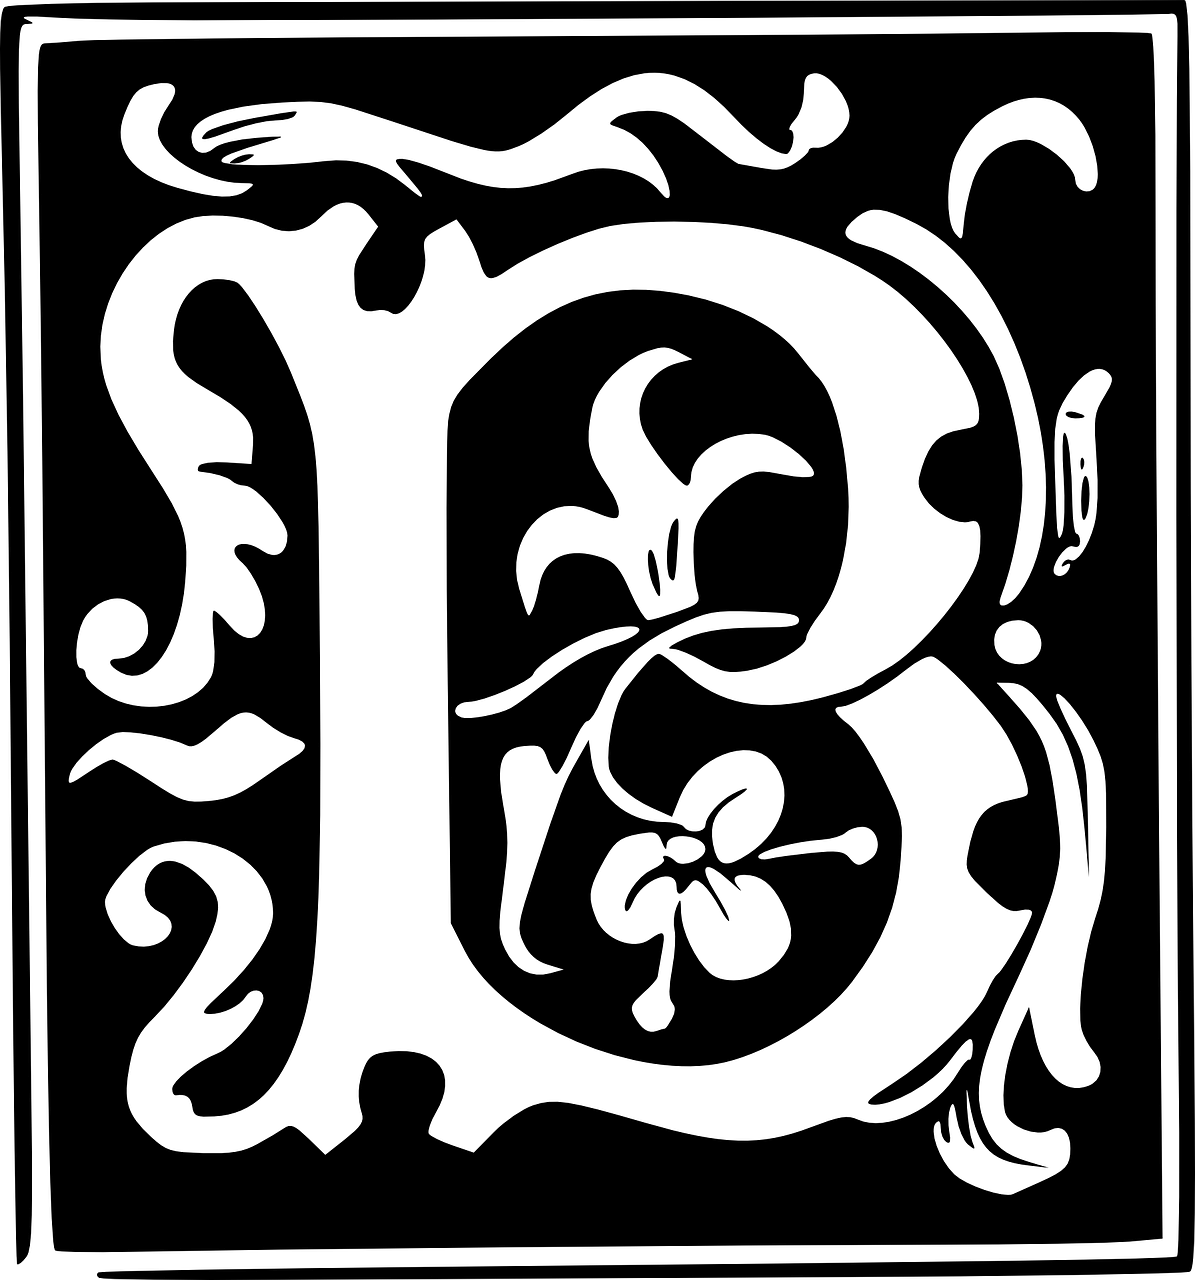
\includegraphics[width=\textwidth]{FancyB.png}
    \caption{A fancy letter B.}
    \label{fig:second}
\end{subfigure}
\caption{A figure with two subfigures.}
\label{fig:doublefigure}
\end{figure}

\newpage
\subsection{Example Subsection With Table}

Here is an example of a table. Note that caption of the table is written with initial capitals, like  a Section or Subsection, and note that it doesn't end with a period as figure caption. Also, the caption is above the table.  You can achieve this by put \verb#\caption{}# command all the way on the top.  You might need to forcibly add space between the text and the table so that it doesn't appear too close to the text.  View the file \texttt{table.tex} for details of the table.
\vspace{4mm}

\renewcommand{\baselinestretch}{0.8}
\newcommand{\PreserveBackslash}[1]{\let\temp=\\#1\let\\=\temp} 
\let\PBS=\PreserveBackslash
\begin{table}[htbp]
\centering
\begin{minipage}{0.89\textwidth}
\caption[Major Differences Between Neural Networks and Cell Signaling Networks]{Major Differences Between Neural Networks and Cell Signaling Networks\protect\footnote{You can also have footnote in table as in figure.}}
\vskip .25in
\label{table:NN_DIFF}

  \footnotesize
    \begin{tabular}
	{|p{0.04 \textwidth}
	|p{0.15 \textwidth}
	|p{ 0.35 \textwidth}
	|p{ 0.35 \textwidth}|} \hline
	\rule{0pt}{1pt} & & & \\
	\strut & 
		\PBS\raggedright{\em Salient features of networks} &
		\PBS\raggedright{\em Neural Networks} &
		\PBS \raggedright{\em Cell Signaling Networks}\\
	\rule{0pt}{1pt}& & & \\ \hline
	\rule{0pt}{1pt}& & & \\
	\strut (i)  & 
		\PBS\raggedright{nodes} & 
		\PBS\raggedright{all nodes typically identical} &
		\PBS\raggedright{nodes are not all equivalent in performance} \\
	\rule{0pt}{1pt}& & & \\ \hline
	\rule{0pt}{1pt}& & & \\
	\strut (ii) & 
		\PBS\raggedright{structure} &
		\PBS\raggedright{typically layered with feed-forward connections only} &
		\PBS\raggedright{regulatory signals often give rise to feedback connections resulting in cycles} \\
	\rule{0pt}{1pt}& & & \\ \hline
	\rule{0pt}{1pt}& & & \\
	\strut (iii) & 
		\PBS\raggedright{connectivity} & 
		\PBS\raggedright{highly connected} &
		\PBS\raggedright{more sparsely connected} \\
	\rule{0pt}{1pt}& & & \\ \hline
	\rule{0pt}{1pt}& & & \\
	\strut (iv) &  
		\PBS\raggedright{learning rule} &
		\PBS\raggedright{connectivity altered to perform a single function e.g.,~via a back-propagation algorithm} &
		\PBS\raggedright{cells must be able to respond to multiple stimuli effectively;changes typically occur via evolutionary processes} \\

	\rule{0pt}{1pt}& & & \\ \hline
    \end{tabular}
\\
\end{minipage}
\end{table}
\renewcommand{\baselinestretch}{1.65}



\begin{equation}
x^2+1
\end{equation}



%%%%%%%%%%%%%%%%%%
%    Appendix    %
%%%%%%%%%%%%%%%%%%

\appendix
% If only one appendix follow the example in appendix.tex.
\oneappendix{Cell Signaling and Stuff}
\label{APP:A}

NJIT has an interesting rule about appendices. If you have more than one appendix, they should be numbered like A, B, and C. These are declared with the \verb#\chapter# command. See the files \texttt{appendixA.tex} and \texttt{appendixB.tex}.

However, if you have only one appendix, it should not be numbered. Removing the number manually leads to all sorts of problems in numbering. equations/figures/tables.  In order that numbering works properly, we have created the \verb#\oneappendix# command that will handle all this for you. Note that's what is used above.

Here's an interesting requirement about NJIT disserations! There has to be text at the beginning of the appendix before any figures or tables. Who knew?

\begin{align}
x^2+1 & = y.\\
x-1 & = y^2.
\end{align}

\begin{figure}[htbp]
\centering

\includegraphics[width=.5in]{msgcube}
\caption{Here's the MSG logo again.}
\label{fig:2} 
\end{figure}


\begin{figure}[htbp]
\centering

\includegraphics[width=.5in]{msgcube}
\caption{Once more with the MSG logo.}
\label{fig:3} 
\end{figure}

\vspace{0.5in}
\renewcommand{\baselinestretch}{0.8} %Change some spacing
{\ssp
\begin{table}[htbp]

\caption{Useful internet sites for cell signaling and protein structure.}
\label{table:WEBSITES}

\begin{center}
	\begin{tabular}
	{|p{0.2in}|
	p{2.5in}|
	p{2.7in}|} \hline 
		\rule{0pt}{1pt} & & \\
			~ & 
			\PBS\raggedright{{\em Web Site} (Cited March 25, 2001)} & 
			\PBS\raggedright{\em Description}  \vspace{1mm} \\ \hline
		\rule{0pt}{1pt} & & \\ 
			$1.$ & 
			\PBS\raggedright{http://vlib.org/Science/ Cell$\_$Biology/ signal$\_$transduction.shtml} &
			\PBS\raggedright{The WWW Virtual Library: Cell Biology---with 
				information on other signal transduction sites of interest} \vspace{1mm}\\
			$2.$ &
			\PBS\raggedright{http://www.grt.kyushu--u.ac.jp/spad/}  &
			\PBS\raggedright{Signaling Pathway Database--- contains diagrams of cell signaling pathways}  \vspace{1mm} \\
			$3.$ &
			\PBS\raggedright{http://geo.nihs.go.jp/csndb/} &  
			\PBS\raggedright{Cell Signaling Networks Database---a signal transduction database \cite{CSND:1999}} \vspace{1mm} \\
			$4.$ &
			\PBS\raggedright{http://www.sdsc.edu/kinases/} &
			\PBS\raggedright{The Protein Kinase Resource---data available on the enzymology, 
				genetics, molecular and structural properties of protein kinases \cite{PKR:1997}} \vspace{1mm}\\
			$5.$ &
			\PBS\raggedright{http://www.expasy.ch/sprot/}  & 
			\PBS\raggedright{SWISS PROT Database---contains protein 
				sequences with functional and structural information \cite{BAIROCH:2000}} \vspace{1mm} \\
			$6.$ &
			\PBS\raggedright{http://www.expasy.ch/prosite/} & 
			\PBS\raggedright{Prosite Pattern Database---contains 
				information on protein families and protein domain structure \cite{HOFMANN:1999}} \vspace{1mm}\\
			$7.$ &
			\PBS\raggedright{http://www.cbs.dtu.dk/databases/ PhosphoBase} &
			\PBS\raggedright{PhosphoBase---a database of phosphorylation sites in proteins \cite{KREEGIPUU:1999}}\vspace{1mm} \\
			$8.$ &
			\PBS\raggedright{http://www--lmmb.ncifcrf.gov/ phosphoDB}    & 
			\PBS\raggedright{Phosphoprotein Database---site dedicated to protein phosphorylation} \vspace{1mm} \\
			$9.$ &
			\PBS\raggedright{http://www.rcsb.org/pdb} & 
			\PBS\raggedright{PBD Brookhaven Crystallographic Database---a protein data 
				bank containing 3--d structural X-ray crystallographic data \cite{BERMAN:2000}} \vspace{1mm} \\
			$10.$ &
			\PBS\raggedright{http://www--nbrf.georgetown.edu/} & 
			\PBS\raggedright{Protein Information Resource--- maintains a protein sequence database, the PIR-International
				Protein Sequence Database \cite{BARKER:2001}} \vspace{1mm}\\
			$11.$ &
			\PBS\raggedright{http://www.ncbi.nlm.nih.gov/} & 
			\PBS\raggedright{National Center for Biotechnology Information} \vspace{1mm} \\ 
			$12.$ &
			\PBS\raggedright{http://www.ncgr.org/software/ pathdb} & 
			\PBS\raggedright{PATHDB: Metabolic Pathways Database---contains information on
			pathways relating to metabolism in plants.} \vspace{1mm} \\ \hline 
				
	\end{tabular}
\end{center}
\end{table}
\endsinglespace}
\renewcommand{\baselinestretch}{2} % Change the spacing back


% If multiple appendices, follow the examples in appendixA.tex and appendixB.tex
%\chapter{Technical stuff}
This section contains material too technical for the average reader. I'm not sure you're qualified to read it.
%\chapter{Very technical stuff}
If you thought the previous section was technical, get a load of what's in this section
$$
e^{i\pi}+1=0.
$$


%%%%%%%%%%%%%%%%%%
%    bibliography    %
%%%%%%%%%%%%%%%%%%

\clearpage

\addcontentsline{toc}{chapter}{REFERENCES}
%\nocite{*}
\printbibliography[title={References}]

\end{document}